\chapter{Analysing Language Models: Foundations, Methods, and Tools}
\label{chapter:analysis-background}

Understanding how language models learn, represent, and generalise linguistic knowledge requires a diverse set of analytical approaches. This chapter surveys foundational work in three interrelated areas: (1) attention-based and representational interpretability, (2) mechanistic interpretability that aims to reverse-engineer internal computations, and (3) learning dynamics research that tracks how capabilities emerge over time during training. 

My emphasis is on methodologies that provide insight into the internal mechanisms of transformer-based models and on tools that help understand developmental trajectories of models. Throughout the chapter, I highlight key techniques for probing attention heads, decomposing learned circuits, tracking convergence and capacity usage, and analysing models across training checkpoints and scales.

I also introduce the growing ecosystem of open-source model suites that enable this research. These tools will form the empirical and methodological foundation for the contributions in the next chapters, where I analyse how small models diverge from larger ones and propose new tools that improve the scientific development of small models. Again, for clarity, key terms and concepts are \thesishl{highlighted} in this chapter.

\section{Attention Analysis and Probing}

The transformer architecture \citep{vaswani2017attention} brought the attention mechanism to the forefront of representation learning. Early efforts to interpret these models focused on analysing attention patterns and probing hidden representations to uncover what linguistic information models capture and how it is distributed across their components.

\subsection{Multi-Head Attention Analysis}

Immediately after the introduction of the transformer architecture, researchers focused on analysing attention patterns to understand how language models represent and process information. A foundational study by \citet{voita2019analyzing} showed that attention heads in transformer models often specialise in distinct linguistic roles, such as syntactic dependencies, coreference, and discourse relations. This head-level specialisation suggested that different attention heads implicitly divide up the task of language processing. They also demonstrated that many heads could be pruned with minimal impact on downstream performance, suggesting that only a subset are essential. \citet{michel2019sixteen} expanded on these findings by measuring redundancy among attention heads. They showed that despite being designed for parallel attention, many heads capture overlapping information. Building on these analytical approaches, \citet{clark2019does} developed visualisation methods for interpreting attention in BERT. In particular, they used the attention weights to visualise the syntactic and semantic relationships in the model. Their study found that BERT's attention heads capture both syntactic and semantic relationships, for instance, tracking subject-verb agreement or coreference chains. Visualising attention remains a widely used diagnostic tool in transformer research. 

\subsection{Sparse Probing}

While attention-based methods offer a window into model behaviour, other approaches have investigated how linguistic structure is embedded in hidden representations. \citet{hewitt2019structural} introduced a structural probe to test whether contextual embeddings encode syntactic information such as dependency trees. Their results showed that BERT's middle layers encode rich syntactic structure in a geometrically meaningful way within the model's representational space. More recently, \citet{gurnee2023finding} proposed sparse probing. This technique constrains linear probes to use only a small number of weights, enforced via $L_0$ regularisation. Their results suggest that linguistic features, although broadly distributed across a model's weights, can be reliably recovered from sparse subsets of weights. %This highlights the potential for localised interpretability, particularly relevant for small models where transparency is more attainable.

\section{Mechanistic Interpretability}

Where sparse probing offers a high-level view of which weights encode linguistic features, mechanistic interpretability aims to reverse-engineer how those features are computed. This approach traces internal mechanisms such as circuits, weights, and layer interactions that give rise to model behaviour. 

\subsection{Foundational Ideas and Circuits}

\begin{figure}[ht!]
    \centering
    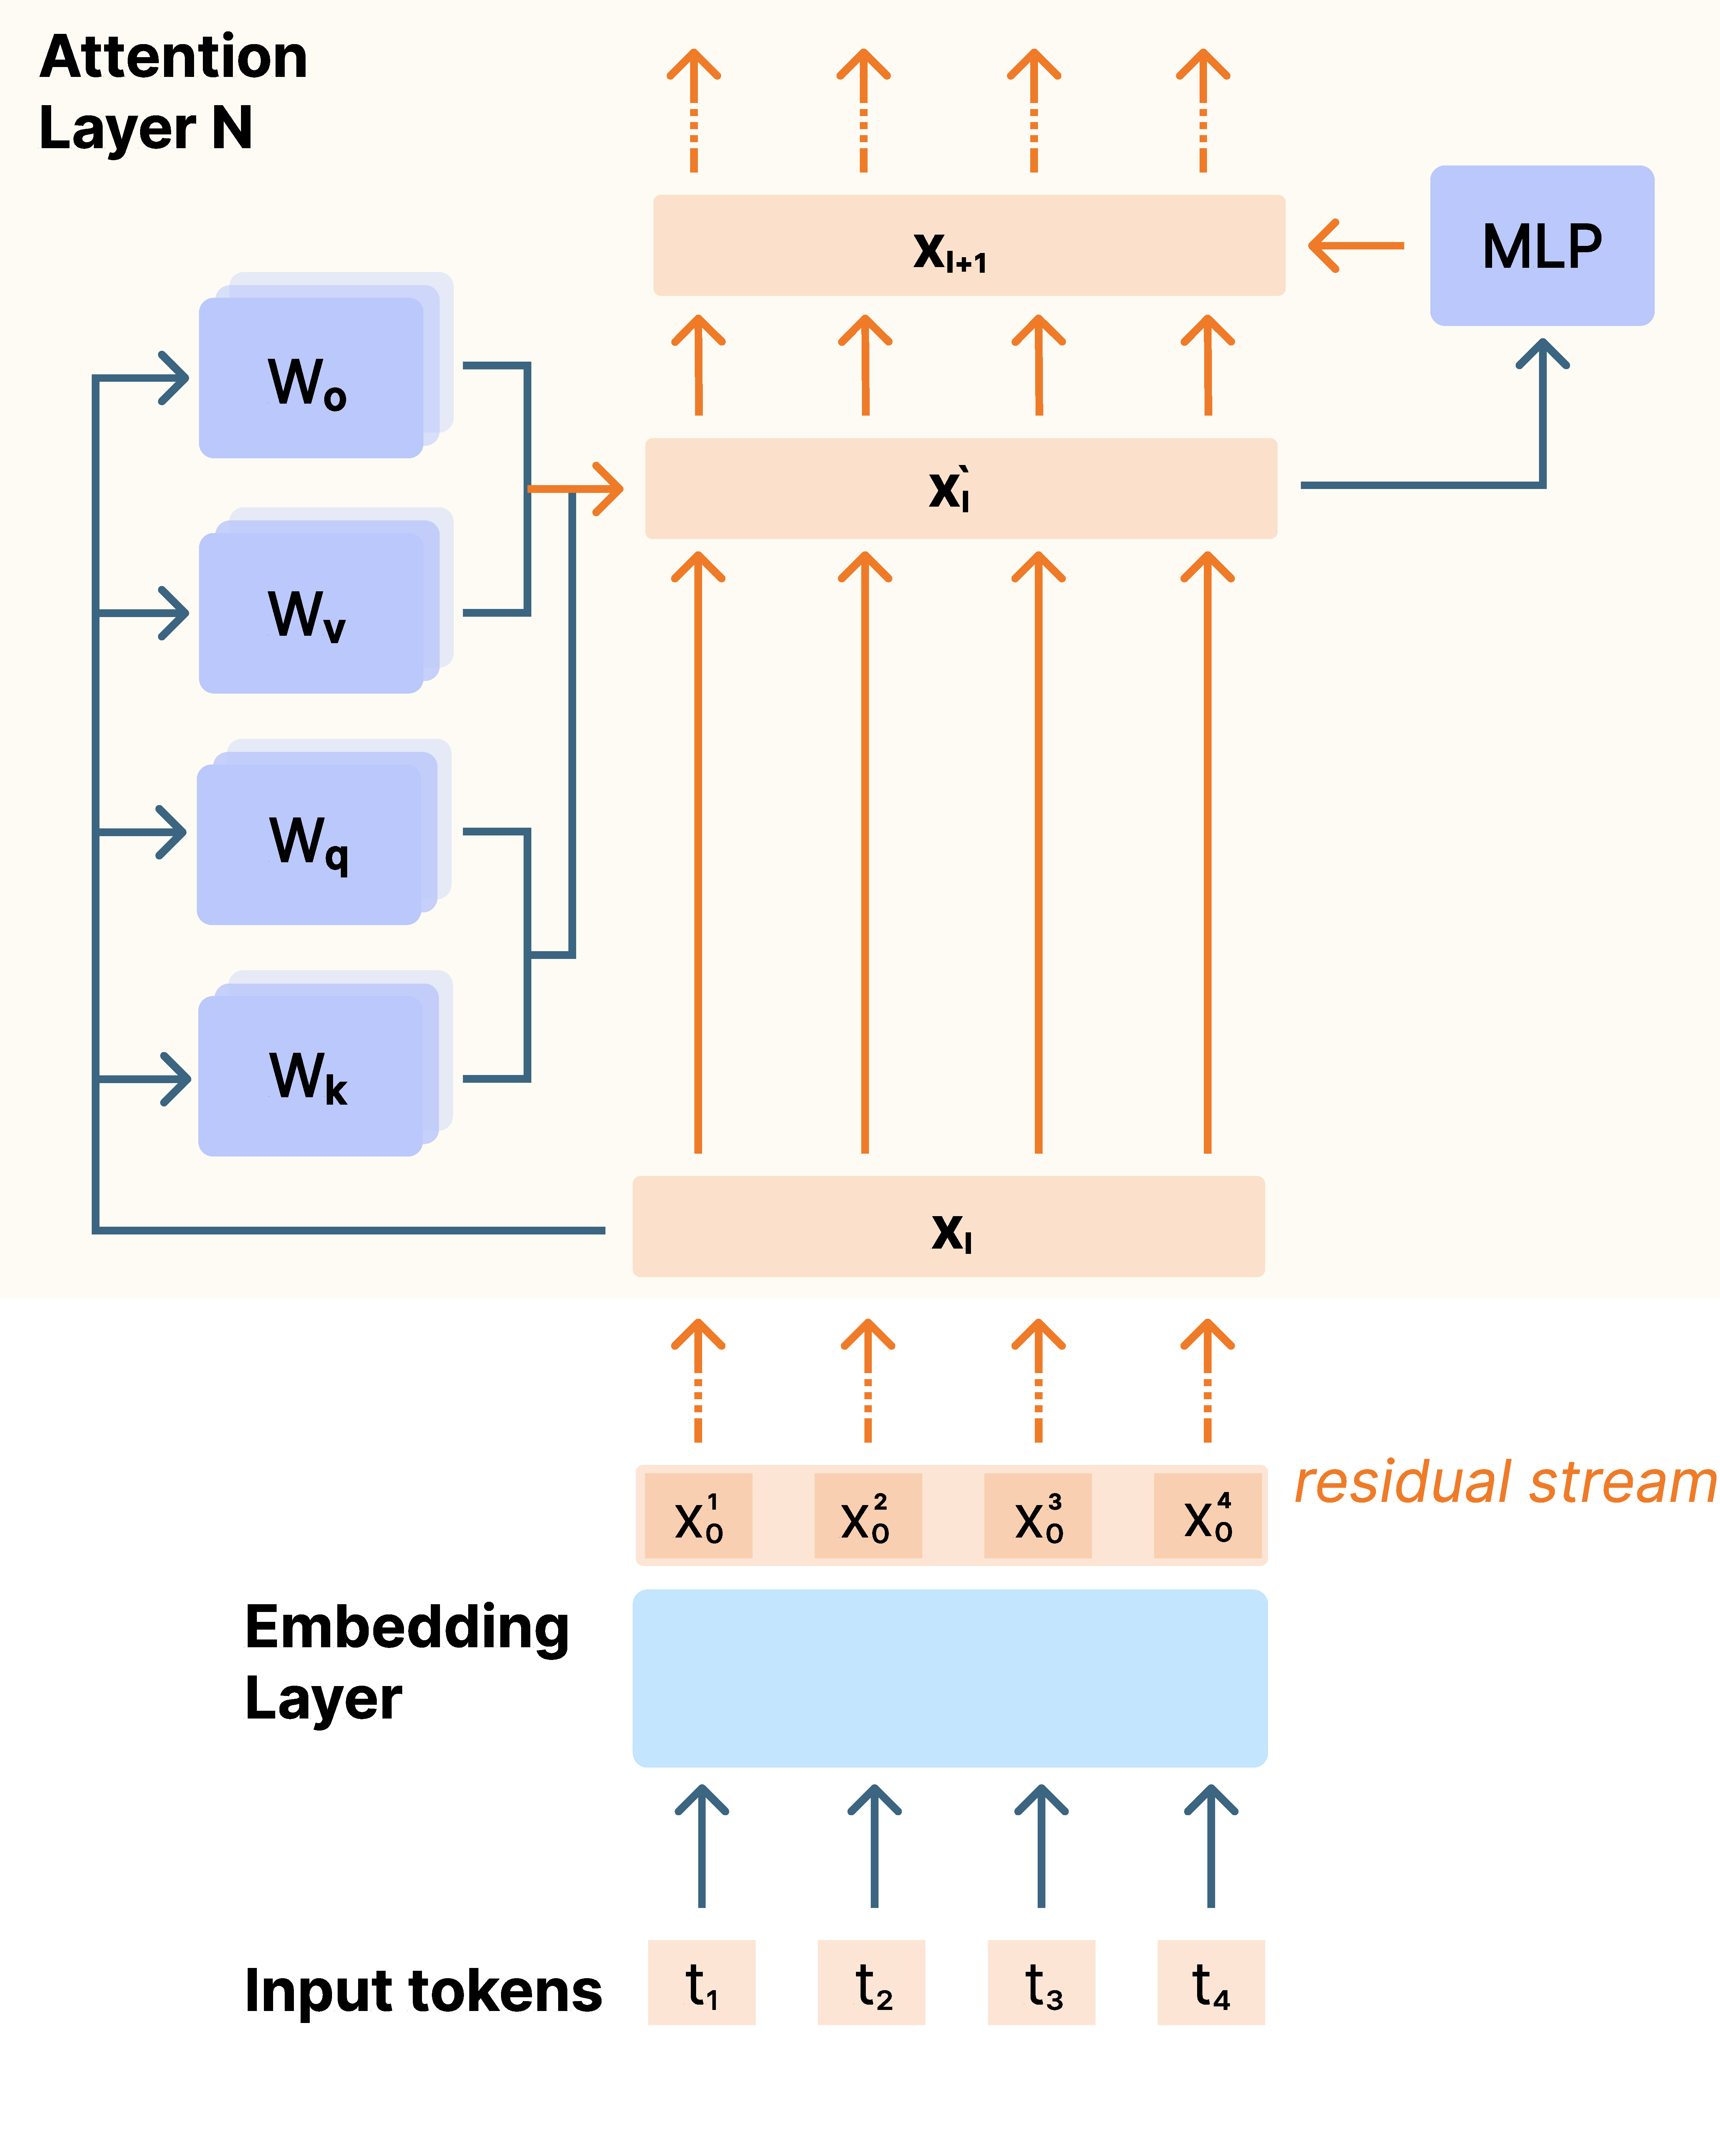
\includegraphics[width=0.6\textwidth]{chapters/analysis_background/figures/residual_stream_visualization.pdf}
    \caption{Visualisation of the residual stream in a transformer model, showing how information flows through the network via skip connections and is progressively refined through attention and feed-forward layers.}
    \label{fig:residual-stream}
\end{figure}


The theoretical foundations of this field were laid by \citet{olah2014manifolds}, who framed neural networks as systems that deform data manifolds while preserving topological structure. This perspective provides a conceptual basis for interpreting how deep models process and transform information layer by layer.

Building on this, \citet{elhage2021mathematical} introduced a formal framework for decomposing transformers into interpretable \thesishl{circuits}. Using tools like “virtual weights,” they showed how specific attention heads can implement distinct algorithms, such as copying text from the context \citep{olsson2022inductionheads}, and how sets of attention heads form structured computational graphs (i.e. circuits) within the model \citep{ameisen2025circuit}. These operations are executed within the shared \thesishl{residual stream}, a central component of transformer architecture that carries forward and combines layer outputs across the model. As illustrated in \cref{fig:residual-stream}, the residual stream serves as the backbone of computation, enabling attention and feed-forward layers to progressively refine and update internal representations at each layer. 
 
Importantly, the residual stream is not a physical entity, but a mathematical formulation that allows us to study the behaviour of the model's internal representations. Under this framework, each of the $L$ layers of a transformer model is thought of as processing a series of input tokens $\sequence = \langle \token_1, \smalldots, \token_\seqlen\rangle$ consecutively and communicates the result of its computation for each token to subsequent layers via a residual stream of dimension $\residualdim$. At each layer, $l$, the current state of the residual stream is denoted as $\xdata_l \in \R^{\seqlen \times \residualdim}$ and represents the model's internal representation of the input sequence at that layer.

The reading, processing, and writing of the residual stream occur independently in each attention head via combinations of the query, key, value, and output matrices, $W_Q$, $W_K$, $W_V$, $W_O$. The \thesishl{query-key circuit}, $W_Q^{\top}W_K$, of the attention mechanism controls how the residual stream should be recomposed, and the \thesishl{output circuit}, $W_OW_V$, writes to the residual stream an update that is mediated by the query-key circuit. The write operation of each attention head is of low rank relative to $\residualdim$. After each attention head has written to the residual stream, a bottleneck \thesishl{Multi-Layer Perceptron (MLP)} projection performs a full-rank transformation on the residual stream. Due to their pivotal role in updating the state of the residual stream, my work in the subsequent chapters analyses the learning dynamics of the two operations that write to the residual stream: the output circuit of each head of the attention layer and the $\mlp$ projection layer.

% A key example of this modular behaviour is the “induction head” described by \citet{olsson2022inductionheads}, which performs in-context learning by detecting repeating token patterns. Their work demonstrated that induction heads are universal across transformer models and emerge consistently during training, highlighting how meaningful algorithmic structure can arise within the residual stream.

\subsection{Applications of Mechanistic Interpretability}

Mechanistic interpretability has been used to study how language models represent and process information. One key insight is that neural networks often represent multiple features in overlapping activation dimensions, a phenomenon known as superposition. \citet{elhage2022toy} formalised this idea and showed how it creates both efficient storage and representational interference. Complementary work by \citet{geva2021memory} reframed feed-forward layers as key-value memory stores, where weights act as retrievable content-addressable memories. This perspective highlights how information retrieval occurs outside the attention mechanism. More recently, \citet{lindsey2025biology} use mechanistic interpretability to analyse complex, higher-order circuits, finding for instance language specific weights in the Claude 3.5 Haiku model \citep{anthropic2024claude3}

Anthropic, the AI company behind Claude \citep{anthropic2024claude3}, is one of the main proponents of mechanistic interpretability, and published much of the aforementioned foundational work in mechanistic interpretability \citep{elhage2021mathematical, elhage2022toy, ameisen2025circuit}. As outlined by the company, Anthropic believe their competitive advantage lies in their ability to fully decompose and identify all the features of language models \citep{anthropic2023components}. To do so, they have popularised the use of sparse autoencoders, a method that trains a small network on top of the features of a language model to reveal what output behaviours of a model are triggered by each feature \citep{templeton2024scaling}. So far, anthropic have catalogued 1000s of features of their models, and are working towards a reserach vision where each parameter's role is fully understood \citep{anthropic2023components}.

\subsection{Tools for Intermediate Layers and Model Analysis}

To support these interpretability efforts, a range of tools and frameworks have emerged.

\citet{belrose2023eliciting} developed the Tuned Lens, a method for interpreting intermediate layers in a model. This approach works by training small linear models to translate the internal activations at each layer into predicted outputs. These predictions are then compared across layers and allow researchers to study how a model's understanding changes across layers.

\citet{nanda2022transformerlens} introduced TransformerLens, a library for inspecting transformer internals, such as attention heads, MLP layers, and residual streams. This library `hooks' into existing models, allowing users to analyse a given model's internal representations and activations. Of all tools in the field, TransformerLens is perhaps the most comprehensive and user-friendly for mechanistic interpretability specifically.

Several tools also support causal and structural interventions. \citet{meng2022locating} proposed ROME, a technique for directly editing factual knowledge in a trained transformer by locating and modifying causal weights. Similarly, \citet{conmy2023towards} developed ACDC, which uses sparse matrix factorisation to automatically extract circuits from models, enabling inference-time interpretability without retraining.

For broader attribution analysis, \citet{kokhlikyan2020captum} developed Captum, a general-purpose library for feature attribution in PyTorch. While not transformer-specific, it includes a suite of interpretability tools, such as Integrated Gradients and DeepLIFT, that are useful for probing feature importance across different model architectures.

% \section{Developmental Interpretability}
% While mechanistic interpretability reveals the internal structure of trained models, developmental interpretability shifts focus to how those structures emerge during training. By analysing checkpoints over time, this approach captures the trajectory of learning—offering insight into when and how linguistic capabilities arise.

% \citet{hoogland2023towards} introduced this paradigm by identifying phase transitions in learning, supported by the Local Learning Coefficient as a measure of representational complexity. Building on this, \citet{hoogland2025losslandscape} connected stagewise learning to loss landscape geometry, revealing that shifts in capability often align with flat or degenerate regions in the optimisation surface.

% To support empirical analysis, \citet{devinterpcode} developed DevInterp, a toolkit for tracking model development over time. Together, these contributions establish developmental interpretability as a powerful complement to static and circuit-based approaches—highlighting not just what models learn, but when and how they acquire it.

% This developmental perspective naturally leads into a broader field of inquiry: learning dynamics—the study of how language models acquire, retain, and organise knowledge over time.

\section{Developmental Interpretability}

While mechanistic interpretability examines the fixed internal structure of trained models, the emerging field of developmental interpretability focuses on how those structures form during training. By analysing model checkpoints over time, it seeks to identify phase changes in learning: that is, abrupt shifts in a model's internal organisation or capability.

\citet{hoogland2023towards} represent a foundational work in this field by introducing the Local Learning Coefficient (LLC), a measure inspired by statistical learning theory. The LLC estimates how quickly a model's effective capacity is increasing at a given point in training, based on local curvature in the loss landscape and parameter dynamics. Building on this, \citet{hoogland2025losslandscape} link stagewise learning to the geometry of the loss surface. Their work shows that capability jumps often occur in flat or degenerate regions where many parameter configurations yield similar performance, and suggests that learning proceeds in bursts of structural change separated by plateaus of fine-tuning. To support such investigations, \citet{devinterpcode} released DevInterp, a toolkit for tracking and visualising model development across training steps.

% In general, developmental interpretability can be seen a new complement to static and circuit-level mechanistic analysis. More generally, however, these are just two, popular methods that fall under the broader umbrella of learning dynamics research.
\section{Learning Dynamics Research}

In general, developmental interpretability and mechanistic interpretability are two, popular methods that fall under the broader umbrella of learning dynamics research. Learning dynamics research investigates the evolving representations and behaviour of models throughout training, using a variety of tools and analytic perspectives. In this section, I survey some of tools that I use in the next chapters to study the learning dynamics of small models.

% \subsection{Memorisation and Data Influence Analysis}
% A central goal in learning dynamics is to understand how specific examples affect learning over time—whether they are memorised, generalised, or forgotten.

% Influence functions, introduced by \citet{koh2017understanding}, trace the effect of individual training examples on model predictions by approximating parameter updates through gradients and inverse Hessians. \citet{grosse2023influence} extended this method to large language models, enabling counterfactual analysis: how would the model behave if a given sequence were added to the training set?

% Complementary to this, prediction trajectory methods analyse how model outputs evolve across training steps. \citet{toneva2019empirical} introduced the concept of forgetting events—when a model switches from correct to incorrect on a training example—offering a lens on stability and difficulty. \citet{swayamdipta2020dataset} expanded this idea with dataset cartography, classifying examples by prediction confidence and variability to map learning trajectories across NLP datasets.
% \citet{feldman2020does} examined the tradeoff between memorisation and generalisation, especially in smaller models where memorisation may be necessary for strong performance. \citet{biderman2023emergent} investigated verbatim memorisation in the Pythia model suite, finding that early checkpoints can effectively forecast what large models will eventually memorise—though smaller models cannot.

% Together, these approaches reveal that memorisation is shaped by training dynamics, model scale, and the specific properties of the data.

\subsection{Convergence and Representation Similarity}

Convergence analysis studies the evolution and stabilisation of internal representations of models during training. This research area seeks to understand when and how model layers begin to encode stable linguistic abstractions, how representational structures develop over time, and the extent to which different models (trained on the same or different data) develop similar internal solutions.

\subsubsection{Measures of Representational Similarity}

One basic heuristic to measure network similarity is `model stitching'. This method investigates whether different models are \textit{functionally} equivalent at certain layers. Originally proposed by \citet{lenc2015understanding} for convolutional networks, this method was later formalised by \citet{bansal2021stitch} as a technique for connecting the lower layers of one model to the upper layers of another, using a small trainable adapter in between. If the stitched model performs well, it suggests that the internal representations of the two models are sufficiently aligned to be interoperable. However, stitching is a coarse signal of similarity, since the performance of the stitched model does not reveal the degree or nature of the representational alignment.

A foundational family of analytically-grounded methods for measuring representational similarity in this space builds on Canonical Correlation Analysis (CCA). CCA is a statistical method that finds linear projections of each representation such that the resulting components are maximally correlated; this provides a measure of how much shared structure exists between the two sets of features. In neural networks, this allows researchers to quantify the alignment between layer activations at different checkpoints, across different models, or within different layers of the same model. \citet{raghu2017svcca} introduced \thesishl{Singular Vector CCA (SVCCA)}, which first reduces the dimensionality of representations via singular value decomposition before applying CCA to the resulting principal components. The output SVCCA measures how correlated the singular values of two representations are, and is a more robust measure of similarity than simple CCA. However, SVCCA has limitations in terms of sensitivity and interpretability.

To address these limitations, \citet{morcos2018pwcca} proposed Projection-Weighted CCA (PWCCA), which weights the contribution of each component according to how much it aligns with the original data. This technique down-weights noisy or low-signal components, yielding a more faithful measure of similarity. Despite these refinements, CCA-based methods still struggle in settings where the representation dimensionality exceeds the number of datapoints; this is nearly always the case in large-scale models that contain high-dimensional embeddings.

To overcome this, \citet{kornblith2019cka} introduced \thesishl{Centred Kernel Alignment (CKA)}, a method based on kernel similarity that offers greater robustness across dimensional regimes. In its linear form, where the kernel is simply the dot product, CKA computes the similarity between two activation matrices \( X, Y \in \mathbb{R}^{n \times d} \) as:

\[
\mathrm{CKA}(X, Y) = \frac{\| Y^\top X \|_F^2}{\| X^\top X \|_F \cdot \| Y^\top Y \|_F}
\]

where \( \|\cdot\|_F \) denotes the Frobenius norm, which for a matrix is the square root of the sum of the squares of all entries. This form of CKA is invariant to orthogonal transformations (e.g., rotations and reflections of the feature space) and isotropic scaling (multiplying all features by the same constant). These properties make CKA particularly well-suited for comparing internal representations across different models, architectures, or training stages.
 
\subsubsection{Applications to Language Models}

These methods have been extensively applied to language models to understand the progression and stability of learned representations. For instance, \citet{saphra2019understanding} used SVCCA to track the alignment of ELMo's hidden states with syntactic annotations, finding that parts-of-speech (POS) information is learned early in training and primarily encoded in lower layers. Similarly, \citet{singh2019bert} applied CCA to multilingual BERT and discovered that representations in the deeper layers diverge across languages and form language-specific clusters.

More recent work by \citet{nguyen2020wide} and \citet{phang2021finetuned} used CKA to identify `block structure' within deep transformers, where layers cluster into groups that share similar representations. These structures are especially pronounced in larger models and later in training, where adjacent layers often encode similar abstractions. \citet{wu2020similarity} found that models from the same architecture family tend to exhibit stronger representational similarity, even if individual weights vary. Finally, \citet{brown2023understanding} analysed intra- and inter-model similarity within the Pythia model suite, using CKA to identify both convergence points and divergence in representation trajectories over time. Their findings support the idea that convergence is not uniform across training but rather unfolds in stages that reflect changes in capacity utilisation, generalisation, and abstraction.

In summary, convergence analysis provides a global view of how language models evolve during training, particularly at the level of their internal representations. Techniques such as CKA, PWCCA, and model stitching offer complementary insights into how and when models develop aligned representations, how stable those representations are, and to what extent learned abstractions are transferable. In the following chapters, I use these tools to study the learning dynamics of small models as a guide for diagnosing inefficiencies, or bottlenecks in training.

\subsection{Sparsity and Norms Analysis}

While convergence analysis provides a high-level view of how internal representations stabilise over time, another important dimension of learning dynamics is how models manage and allocate their \thesishl{capacity}: that is, the number of different complex `functions' or more broadly patterns a model can learn. Analyses of \thesishl{sparsity} and \thesishl{norms} offer fine-grained insight into how models compress information over the training process.

%This line of work investigates not only how sparsity emerges during training, but also how different types of norms—such as activation norms, weight norms, and gradient scales—fluctuate and influence model behaviour. Together, these metrics help reveal how language models balance expressivity with efficiency and stability.

\subsubsection{Sparsity Metrics and Analysis}

A sparse matrix is defined as a matrix with many zero entries. In the context of a neural network, sparsity measures how many of the model's parameters are `close' to zero.

A foundational contribution to the measurement of sparsity came from \citet{hoyer2004sparsity}, who proposed a continuous sparsity score that combines the \( \ell_1 \) and \( \ell_2 \) norms of a vector. This \thesishl {Hoyer's sparsity} metric ranges from 0 (fully dense) to 1 (maximally sparse), making it particularly effective for tracking the emergence of sparse representations in activation maps or weight matrices during training.

\citet{hurley2009gini} evaluated various sparsity measures from a theoretical perspective, outlining six desirable properties such as scale and permutation invariance. They highlight the \thesishl{Gini coefficient}, a metric from the field of econometrics, as a particularly useful measure that satisfies these properties. The Gini coefficient quantifies inequality in a distribution by measuring the average absolute difference between all pairs of values, normalised by the mean of the distribution \citep{hurley2009gini}. In the context of neural networks, it can be applied to weight vectors or activation patterns to capture the unevenness of magnitude across elements.
 
% \subsubsection{Functional Sparsity in Language Models}

% Beyond abstract metrics, several studies have explored `functional sparsity': how neural models naturally deactivate or underutilise certain components during training. \citet{frankle2019lottery} introduced the \textit{lottery ticket hypothesis}, showing that sparse subnetworks within overparameterized models can achieve full performance if trained in isolation. This finding sparked a wave of interest in understanding which parameters are actively contributing to learning and which are not.

% Building on this, \citet{michel2019sixteen} found that many attention heads in transformers can be pruned without degrading performance—suggesting redundancy in head usage and an opportunity for model compression. \citet{voita2019analysing} confirmed this by introducing \textit{head importance scoring}, showing that some attention heads specialise in interpretable functions while others effectively deactivate, illustrating emergent sparsity during training.

% \citet{evci2020rigging} analysed the training trajectories of sparse networks and found that early training phases are especially unstable when sparsity is enforced too aggressively. This underscores the importance of understanding when sparsity is beneficial and how it interacts with training dynamics.

% More recently, \citet{jiang2023pruning} proposed sparsity-aware pruning strategies tailored to pretrained transformers, focusing on neurons that become saturated, unused, or ``dead'' over the course of training. Their work provides practical tools for diagnosing inefficiencies in model capacity usage.

\subsubsection{Norm Evolution and Training Stability}

Complementing sparsity analysis, research into \thesishl{norm dynamics} offers insight into the scaling and stability of model parameters and activations. In the context of this thesis, most norms discussed are \thesishl{matrix norms}. In general, a matrix norm is a function that assigns a non-negative scalar to a matrix that quantifies its size in a way that satisfies non-negativity, positive homogeneity, and the triangle inequality. Different norms capture different structural aspects of the matrix. Common choices include:

\begin{itemize}
    \item \textbf{$\ell_1$ norm}: the maximum absolute column sum,
    \[
    \|\mathbf{A}\|_1 = \max_{1 \leq j \leq n} \sum_{i=1}^m |a_{ij}|,
    \]
    which reflects the largest accumulated magnitude along any column.
    \item \textbf{$\ell_\infty$ norm}: the maximum absolute row sum,
    \[
    \|\mathbf{A}\|_\infty = \max_{1 \leq i \leq m} \sum_{j=1}^n |a_{ij}|,
    \]
    highlighting the largest row-wise contribution.
    \item \textbf{Frobenius norm}: the square root of the sum of squared entries,
    \[
    \|\mathbf{A}\|_F = \sqrt{\sum_{i=1}^m \sum_{j=1}^n a_{ij}^2},
    \]
    analogous to the $\ell_2$ norm for vectors and sensitive to the overall energy of the matrix.
    \item \textbf{Spectral norm}: the largest singular value of $\mathbf{A}$,
    \[
    \|\mathbf{A}\|_2 = \sigma_{\max}(\mathbf{A}),
    \]
    which measures the maximum amplification factor of the matrix when acting as a linear transformation.
\end{itemize}

Norms are useful to understand the scaling of model parameters and activations over the training process. For example, \citet{mishkin2016goodinit} studied how weight and activation norms evolve during training and highlighted the role of proper initialisation and normalisation (e.g., LayerNorm) in maintaining stable learning. Their findings are particularly relevant in transformer architectures where residual pathways can lead to norm drift. \citet{liu2020understanding} examined gradient and activation norm instability in transformers, identifying early-phase training as especially vulnerable to vanishing or exploding norms. From a theoretical angle, \citet{arora2018theoretical} connected parameter norm growth to generalisation bounds, suggesting that norm-based proxies can signal overfitting or underfitting. These instabilities can explain training failures and motivate adjustments to, for example, learning rates or normalisation strategies. 

\subsection{Effective Rank Analysis}

Beyond sparsity and norms, understanding how many dimensions a model \textit{actually uses} to represent information reveals important dynamics of learning and capacity utilisation. While a given model might in theory have a large number of parameters, recent work has shown that models often use only a small fraction of their capacity. In this thesis, I explore metrics that quantify a model's effective capacity.

Training often unfolds in distinct stages that is marked by shifts in representational rank. \citet{boix-adsera2023rank} showed that transformer weights increase in rank incrementally from initialisation, mirroring stepwise acquisition of complexity. This is further supported by \citet{belrose2024neural}, who observed that models progressively encode more sophisticated statistical patterns, starting from unigrams and advancing towards complicated syntax. These dynamics are particularly relevant for small models. \citet{godey2024small} found that small language models hit a representational bottleneck at the output layer: the softmax saturates in rank even while loss continues to fall. This suggests underperformance may stem from expressivity ceilings, not optimisation failure.

To characterise these dynamics, researchers have proposed several ways to estimate how many dimensions a model functionally uses. 

One simple, approximate metric is the \thesishl{condition number} of a matrix. The condition number of a matrix $A$ measures how sensitive its output is to small changes in the input, and is defined as the ratio of its largest to smallest singular value:
\[
\kappa(A) = \frac{\sigma_{\max}(A)}{\sigma_{\min}(A)}.
\]
A low condition number (close to $1$) indicates that all dimensions are scaled similarly, while a high condition number suggests that some directions in the space are much more amplified or attenuated than others. In the context of representation analysis, a high condition number implies that the model's representation is effectively confined to a narrow subspace, even if the nominal rank is high.

\citet{garg2025utilizedrank} introduced utilised rank, which estimates the number of active dimensions in a layer's weight matrix by projecting it onto input/output subspaces derived from real data. Their analysis showed that many large models use only a small fraction of their nominal capacity; for example, ViT-L/16 utilises just $\sim$20\% of its available rank.

Another approach is \thesishl{effective rank} (ER), a continuous measure of dimensionality based on the entropy of a matrix's singular values \citep{roy2007effectiverank}. Given singular values $\sigma_1, \dots, \sigma_r$, normalised as $p_i = \frac{\sigma_i}{\sum_j \sigma_j}$, of a matrix $\mathbb{A}$, the effective rank is defined as:

\[
\mathrm{ER}(A) = \exp\left(-\sum_{i=1}^r p_i \log p_i\right)
\]

This metric ranges from 1 (collapsed representation) to $r$ (full rank), offering a smooth, interpretable way to track representational complexity. I adopt this measure in later chapters to analyse the learning dynamics of small language models.

% Multiple studies have observed discrete jumps in effective rank, closely aligned with drops in training loss—a phenomenon termed the \textit{rank staircase} by \citet{yang2024rankstaircase}. These transitions mark key inflection points in the learning process, supporting the idea that training progresses in qualitatively distinct stages.

% More broadly, rank-based analyses suggest that low-rank structure is an emergent property of training itself. \citet{pellegrino2023lowrank} found that both biological and artificial networks tend to evolve along low-dimensional subspaces. \citet{feng2022rank} and \citet{minyoung2022lowrank} provide theoretical support, showing that neural networks exhibit a bias toward rank-deficient representations and structurally simple solutions.

In sum, effective rank analysis deepens reseachers' understanding of how language models acquire, and allocate representational capacity. Later chapters build on this foundation, using effective rank to study capacity bottlenecks and phase transitions in small model training.

\section{Model Suites for Learning Dynamics Research}

Understanding how language models learn requires visibility into the training process itself. This is especially critical when comparing how models of different sizes acquire capabilities, converge to solutions (or fail to do so). To study these differences, researchers increasingly rely on \thesishl{model suites} which are families of models trained across a range of scales that all use the same architecture, training procedure and data for ideal apples-to-apples comparisons. Importantly, these suites are often released with intermediate checkpoints, logs, and other training metadata, allowing for fine-grained post-hoc analysis of model behaviour over time.

% This section surveys a set of frameworks that make such investigations possible. These resources are essential for answering \textbf{Research Question 2:} \textit{How can we more quantitatively understand how small models learn and what makes them different from large models?} By enabling cross-scale comparisons, these tools help reveal when and why smaller models diverge, and support targeted hypotheses for making their learning dynamics smoother and more effective.

\subsection{Comprehensive Model Suites with Scale Transparency}

One of the most widely used resources for studying learning dynamics is \thesishl{Pythia} \citep{biderman2023pythia}, a suite of 16 decoder-only language models ranging from 70M to 12B parameters. Each model includes 154 training checkpoints, enabling fine-grained analysis across both time and scale. Pythia has become a standard resource for studying memorisation, convergence patterns, and representational development in autoregressive transformers \citep{lesci2024causal,godey2024anisotropy,belrose2023eliciting}.

OLMo \citep{groeneveld2024olmo} is a newer model suite that is trained on larger datasets than Pythia. It includes several 7B-parameter models and a 1B model, all trained on 2T tokens with full access to training logs, intermediate checkpoints, and evaluation tools such as Catwalk \citep{groeneveld2023catwalk} and Paloma \citep{magnusson2024paloma}.

Complementing this, BLOOM \citep{le2023bloom} offers a multilingual and globally inclusive model suite. It spans models from 560M to 176B parameters, with public checkpoints released at multiple stages (e.g., 100B, 500B, 1.5T tokens). BLOOM is particularly well-suited for studying cross-lingual representation learning and transfer, making it a valuable resource for multilingual language modelling research.

In parallel, LLM360 \citep{liu2023llm360} takes a radical transparency approach by releasing dense sequences of checkpoints (e.g., 360 for their Amber and 143 for CrystalCoder models) alongside optimiser states, loss curves, and detailed logs. This level of granularity supports fine-grained studies of model robustness, generalisation, and representational change across training.

\subsection{Frameworks for Small Model Interpretability}

Several recent frameworks have focused on smaller, more interpretable models. MobiLlama \citep{thawakar2024mobillama} provides a lightweight GPT-style model trained for mobile uses cases that is fully transparent and reproducible. TinyLlama \citep{liu2023llm360} offers a 1.1B-parameter model trained on 3T tokens, with checkpoints released at regular intervals (105B to 3T tokens). Finally, SmolLM2 \citep{allal2025smollm2} was specifically designed for mechanistic interpretability with native Hugging Face integration, releasing checkpoints every 125K steps from a 1.7B-parameter model. 

\subsection{Implications for Learning Dynamics Research}

Collectively, these frameworks provide the empirical foundation for learning dynamics research by exposing how models evolve over time and across scales. With access to intermediate checkpoints, logs, and multiple model sizes, they enable systematic comparisons of when and how capabilities emerge, and why smaller models often diverge from their larger counterparts.

In the next chapter, I use the Pythia suite to analyse differences in convergence between small and large models, motivating hypotheses about how to encourage smoother learning. Building on these insights, the final chapter introduces \pico, a new framework designed to support efficient, interpretable retraining of small models and accelerate experimental iteration on learning dynamics interventions.
